% copyright by Zhou Lvwen. zhou.lv.wen@gmail.com
\documentclass[12pt,a4paper]{article}   % 文档说明[字号, 纸张类型]{文档类型}
%%%%%%%%%%%%%%%%%%%%%%%%%%%%%% 导 言 区 %%%%%%%%%%%%%%%%%%%%%%%%%%%%%%%%%%%%
\usepackage{amsmath,fancyhdr,graphicx,appendix,lastpage,extramarks,array}
\usepackage{listings}
\usepackage{xcolor}
\usepackage{attachfile2}
% 定义页边距[左  =1in,右   =1in,上 =1.2in,下=1in]
\usepackage[left=0.8in,right=0.8in,top=1.2in,bottom=1in]{geometry}
%%%%%%%%%%%%%%%%%%%%%%%%%%%%%%%%%%%%%%%%%%%%%%%%%%%%%%
\usepackage{xeCJK}
%\usepackage{fontspec}
\setCJKmainfont[BoldFont=simhei.ttf]{simsun.ttf}
%%%%%%%%%%%%%%%%%%%%%%%%%%%%%%%%%%%%%%%%%%%%%%%%%%%%%%
\setlength{\parskip}{2pt}               % 定义段落间距

% 定义页眉: 左页眉{中文姓名, 学号}, 便为老师打分, 所以这里用中文姓名
%           中页眉{英语学术论文写作}为课程名称
%           右页眉{第X页,共X页}
\pagestyle{fancy} \lhead{周吕文, 201128000718065} 
\chead{英语学术论文写作(排版作业)}
\rhead{第\ \thepage\ 页,{~} 共\ \protect\pageref{LastPage} 页}

% 注: 各位同学改改页边距, 段落间距及页眉. 别搞得大家版式一样
%%%%%%%%%%%%%%%%%%%%%%%%%%%%%%%%%%%%%%%%%%%%%%%%%%%%%%%%%%%%%%%%%%%%%%%%%%%%
% Latex code 环境
{\definecolor{MyDarkGreen}{rgb}{0.0,0.3,0.0}
\definecolor{hellgelb}{rgb}{0.96,0.96,0.96}
\usepackage{showexpl}
\lstset
{
    language=[LaTeX]TeX,
    breaklines=true,
    basicstyle=\footnotesize\ttfamily,
    commentstyle=\color{MyDarkGreen}\footnotesize,
    keywordstyle=\color{blue},
    identifierstyle=\color{magenta},
     columns=fixed,
     tabsize=4,%
     frame=single,%
     framerule=1pt,
     extendedchars=true,%
     showspaces=false,%
     showstringspaces=false,%
     numbers=left,%
     numberstyle=\tiny\ttfamily,%
     numbersep=1em,%
     breaklines=true,%
     breakindent=10pt,%
     backgroundcolor=\color{hellgelb},%
     breakautoindent=true,%
     captionpos=t,%
     xleftmargin=1em,%
     xrightmargin=\fboxsep%
}

%%%%%%%%%%%%%%%%%%%%%%%%%%%%%% 正    文 %%%%%%%%%%%%%%%%%%%%%%%%%%%%%%%%%%%%
\begin{document}
\title{The Dissipative Particle Dynamics Simulation of Macromolecular Suspension in Micro-channels}     % 论文标题

% 作者\\单位
\author{ZHOU Lv-Wen$^1$\footnote{zhou.lv.wen@gmail.com}, LIU Mou-Bin$^2$\\          
       \textit{$^{1,2}$Institute of Mechanics, CAS, Beijing 100190, China}}
\date{July 1, 2012}                     % 写作日期, 省略则为当前计算机日期
\maketitle
\thispagestyle{fancy}                   % 首页添加页眉

% .........................................................................
\begin{abstract}                        % 摘要
This paper investigated the transport and conformation of macromolecules in micro-channels using the dissipative particle dynamics (DPD) and finite extensible non-linear elastic (FENE) bead spring chains model. The dynamic behavior of macromolecules with different number of beads and different chain length in three kinds of micro-channels, straight quadrate contraction sloping contraction micro-channel are comparatively analyzed. It is found that the macromolecules tend to drag the simple DPD particles, reducing their velocity, and leading to density fluctuations. The dragging effect is more important as the number of macromolecules or the length of the macromolecular chain increases.
\end{abstract}
% .........................................................................

\section{Introduction}                  % 引言
 Understanding the dynamic behavior of macromolecules, such as DNA, is very important for fundamental research and practical applications in bio, chemical and medical engineering, especially in the designing micro-devices. Recently, micro-devices enable processing, analyzing, and delivering biochemical materials in a wide range of biomedical and biological applications\cite{KChun,FanX}.

%..........................................................................
\section{Methodology of the dissipative particle dynamics}     % 正文
In Dissipative particle dynamics system, a particle is represented a cluster of molecules or small regions of fluid material. The forces between particles are assumed to be pair-wise additive. The motion of DPD particles is governed by Newton's equations of motion. For simple DPD particle $i$ , we have the governing equations
\begin{equation}
\frac{\mathrm{d}r_i}{\mathrm{d}t} = v_i,\,\,\,\,\,
\frac{\mathrm{d}v_i}{\mathrm{d}t} = \sum_{j\neq i}^N f_{ij_{i}}^{\mathrm{ext}}
\end{equation}
Where $r_i$ and $v_i$ denote the position and velocity of particle $i$. The mass of the all DPD particle has been taken to be the same and unity; and $f_{ij}$ denote the total force between particles $i$ and $j$. $f_i^{\mathrm{ext}}$ is the external force, such as the gravity. The inter-particle force $f_{ij}$ consists of three parts, namely: conservative force $F_{ij}^C$, dissipative force $F_{ij}^D$ and random force $F_{ij}^R$.

\begin{equation}
\mathbf{F}_{ij}^{C}=\begin{cases}
a_{ij}(1-r_{ij}/r_{c})\mathbf{\hat{r}}_{ij} & r_{ij}<r_{C}\\
0 & r_{ij}\geq r_{C}
\end{cases}
\end{equation}

\section{Parameters}

To construct a working DPD, we need select values of some necessary parameters. In this section, we will talk abut how to select model parameters' values. Table \ref{parameters} listed the some model parameters that we need determined before we could sufficient to construct a working DPD system. For a simple single component DPD system, we just set all particles' mass to be unity, and cutoff radius is also set to be unity.
\begin{table}[!htb]
\centering
\caption{\label{parameters}Model parameters}
\begin{tabular}{|l|l|l|}
\textbf{Model parameters} & \multicolumn{1}{c|}{\textbf{Symbol}} & \multicolumn{1}{c|}{\textbf{Value}} \\
\hline
Mass of DPD particle & \multicolumn{1}{c|}{$m$} & \multicolumn{1}{c|}{unity} \\
\hline
Cutoff radius of DPD particle & \multicolumn{1}{c|}{$r_C$} & \multicolumn{1}{c|}{unity} \\
\hline
Simulation time step & \multicolumn{1}{c|}{$\Delta t$} & \multicolumn{1}{c|}{} \\
\hline
Friction coefficient & \multicolumn{1}{c|}{$\gamma$} & \multicolumn{1}{c|}{$\sigma=2\gamma k_bT$} \\
\hline
\end{tabular}
\end{table}

\section{Channel flow of FENE chain suspension}

We use DPD particles and FENE chains to model the suspension of macromolecules in three kinds of micro-channels. Quadrate contraction micro-channel and sloping contraction micro-channel are comparatively analyzed. The conformation evolution of macromolecules passing through quadrate contraction micro-channel and sloping contraction micro-channel at $t = 4000$ are show in figure \ref{chainT} and figure \ref{chainY} respectively.

\begin{figure}[!htb]
\centering
\begin{minipage}[c]{0.5\textwidth}
\centering
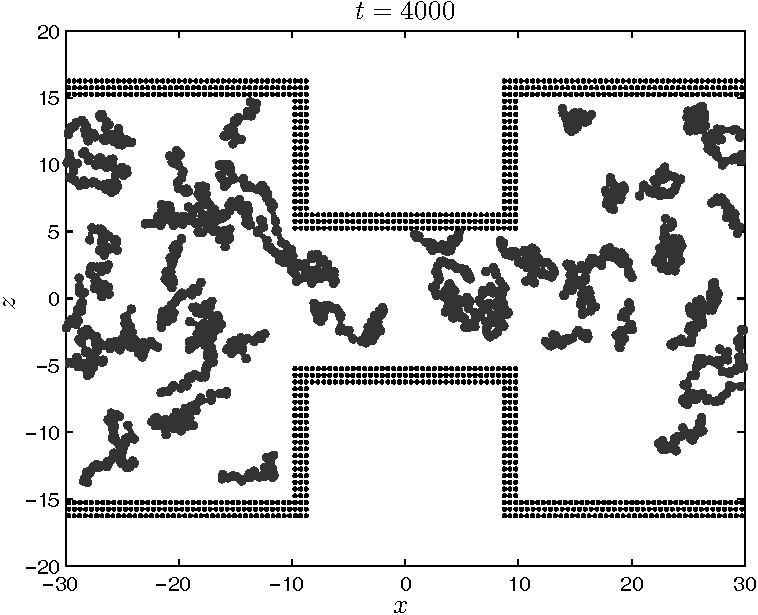
\includegraphics[width=0.85\textwidth]{./figures/chainT4000s.pdf}
\caption{\label{chainT} Quadrate contraction micro-channel}
\end{minipage}%
\begin{minipage}[c]{0.5\textwidth}
\centering
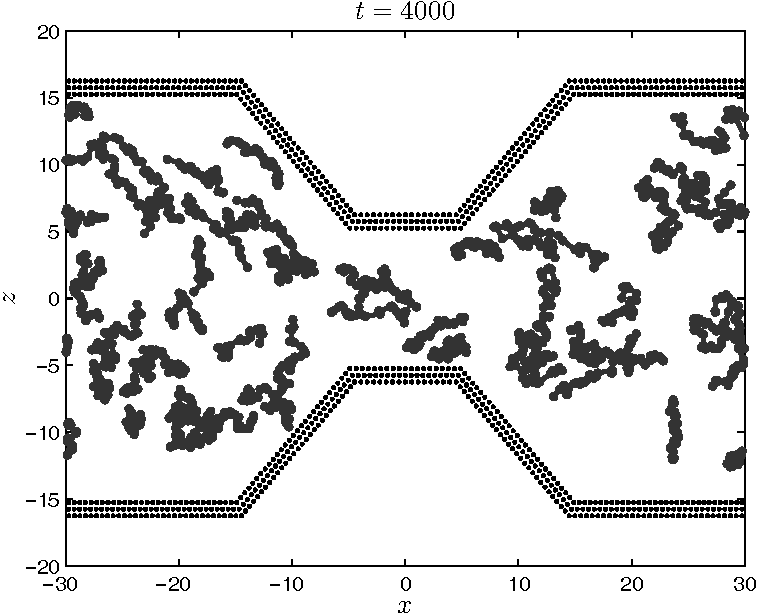
\includegraphics[width=0.85\textwidth]{./figures/chainY4000s.pdf}
\caption{\label{chainY} Sloping contraction micro-channel}
\end{minipage}
\end{figure}

%.........................................................................


\section{Conclusion}                    % 结论
Our numerical results show that macromolecules are mainly concentrated in the middle channel. Macromolecules tend to drag simple fluid particles, reducing their velocity, and leading to density and velocity fluctuations. The dragging effect is more important as the number of macromolecules or the length of the macromolecular chain increases.

The conclusions of this paper is very important for fundamental research and practical applications in bio, chemical and medical engineering. By control the flow of macromolecular suspensions, which carried drugs and DNA molecules, we can efficiently and precisely deliver a small amount of drug or DNA into local tissue, skin regions, and even cells.

%.........................................................................
\section*{Acknowledgements}             % 致谢
I would like to thank LIU Mou-Bin.

%.........................................................................
\begin{thebibliography}{99}             % 参考文献
\bibitem{KChun} K. Chun, G. Hashiguchi, H. Toshiyoshi, and H. Fujita, ``Fabrication of array of hollow microcapillaries used for injection of genetic materials into animal/plant cells,'' Jpn. J. Appl. Phys., Part 2 38, L279(1999).
\bibitem{FanX} Fan X, Phan-Thien N, Yong N T, Wu X, Xu D. ``Microchannel flow of a macromolecular suspension''. Phys Fluids, 2003, 15(1): 11-21
\end{thebibliography}


\newpage
%.........................................................................
\appendix
\appendixpage                           % 附录
\section{\textattachfile[color=red]{main.tex}{Latex Code}}                    % 附录 A
\lstinputlisting{main.tex}
\end{document} 
